%header and footer for separate chapter files

\ifx\whole\undefined
\documentclass[12pt, leqno]{book}
\usepackage{graphicx}
\input style-for-curves.sty
\usepackage{hyperref}
\usepackage{showkeys} %This shows the labels.
%\usepackage{SLAG,msribib,local}
%\usepackage{amsmath,amscd,amsthm,amssymb,amsxtra,latexsym,epsfig,epic,graphics}
%\usepackage[matrix,arrow,curve]{xy}
%\usepackage{graphicx}
%\usepackage{diagrams}
%
%%\usepackage{amsrefs}
%%%%%%%%%%%%%%%%%%%%%%%%%%%%%%%%%%%%%%%%%%
%%\textwidth16cm
%%\textheight20cm
%%\topmargin-2cm
%\oddsidemargin.8cm
%\evensidemargin1cm
%
%%%%%%Definitions
%\input preamble.tex
%\input style-for-curves.sty
%\def\TU{{\bf U}}
%\def\AA{{\mathbb A}}
%\def\BB{{\mathbb B}}
%\def\CC{{\mathbb C}}
%\def\QQ{{\mathbb Q}}
%\def\RR{{\mathbb R}}
%\def\facet{{\bf facet}}
%\def\image{{\rm image}}
%\def\cE{{\cal E}}
%\def\cF{{\cal F}}
%\def\cG{{\cal G}}
%\def\cH{{\cal H}}
%\def\cHom{{{\cal H}om}}
%\def\h{{\rm h}}
% \def\bs{{Boij-S\"oderberg{} }}
%
%\makeatletter
%\def\Ddots{\mathinner{\mkern1mu\raise\p@
%\vbox{\kern7\p@\hbox{.}}\mkern2mu
%\raise4\p@\hbox{.}\mkern2mu\raise7\p@\hbox{.}\mkern1mu}}
%\makeatother

%%
%\pagestyle{myheadings}

%\input style-for-curves.tex
%\documentclass{cambridge7A}
%\usepackage{hatcher_revised} 
%\usepackage{3264}
   
\errorcontextlines=1000
%\usepackage{makeidx}
\let\see\relax
\usepackage{makeidx}
\makeindex
% \index{word} in the doc; \index{variety!algebraic} gives variety, algebraic
% PUT a % after each \index{***}

\overfullrule=5pt
\catcode`\@\active
\def@{\mskip1.5mu} %produce a small space in math with an @

\title{Personalities of Curves}
\author{\copyright David Eisenbud and Joe Harris}
%%\includeonly{%
%0-intro,01-ChowRingDogma,02-FirstExamples,03-Grassmannians,04-GeneralGrassmannians
%,05-VectorBundlesAndChernClasses,06-LinesOnHypersurfaces,07-SingularElementsOfLinearSeries,
%08-ParameterSpaces,
%bib
%}

\date{\today}
%%\date{}
%\title{Curves}
%%{\normalsize ***Preliminary Version***}} 
%\author{David Eisenbud and Joe Harris }
%
%\begin{document}

\begin{document}
\maketitle

\pagenumbering{roman}
\setcounter{page}{5}
%\begin{5}
%\end{5}
\pagenumbering{arabic}
\tableofcontents
\fi


\chapter{Brill--Noether theory and applications to genus 6}\label{Brill--Noether}\label{BNChapter}

\section{What linear series exist?}

Let's start with a naive question: when does there exist a curve $C$
of genus $g$ and a $g^r_d$ on $C$\emdash equivalently, a line bundle
$\cL$ of degree $d$ on $C$ with $h^0(\cL) \geq r+1$? The
Riemann--Roch and
\index{Riemann--Roch theorem}%
Clifford theorems
\index{Clifford theorem}%
together provide a complete answer to this question:

\begin{theorem}\label{arbitrary linear series}
There exists a curve $C$ of genus $g$ and a line bundle $\cL$ of degree $d$ on $C$ with $h^0(\cL) \geq r+1$ if and only~if
$$
r \leq
\begin{tcases}
d-g& \quad \text{if } d \geq 2g-1; \text{ and} \\
d/2&  \quad \text{if } 0 \leq d \leq 2g-2.
\end{tcases}
$$
\end{theorem}


For the
perhaps more interesting question of when  there
exists a curve of genus $g$ with a
birationally very ample $g^r_d$, Castelnuovo's theorem
\index{birationally very ample}%
\index{g@$g^r_d$}%
\index{Castelnuovo's theorem}%
gives a quadratic bound, roughly $d \geq
\sqrt{g(2r-2)}$.

In both these situations, the curves that achieve the bounds are quite
special. Perhaps the most interesting question
is, for which $r,d$ do \emph{all} curves of genus $g$ have a $g^r_d$,
and what is the
behavior of these series on a general curve?
\index{Brill--Noether theory|(}%
Brill--Noether theory
provides some answers to both these questions.

\section{Brill--Noether theory}

The following result was stated by Brill and Noether in 1874, and finally
\index{Brill, Alexander}%
\index{Noether, Max}%
\index{historical context}%
proven in a series of works by
Kempf
\citeyear{Kempf},
Kleiman and Laksov
\index{Laksov, Dan}%
\index{Kleiman, Steven}%
\index{Griffiths, Phillip A.}%
\index{Kempf, George}%
\citeyear{MR323792,MR0357398},
and Kleiman \citeyear{Kleiman-special},
culminating in a paper by
Griffiths and the second author \cite{Griffiths-Harris-BN}.

\begin{theorem}[basic Brill--Noether]\label{basic BN}
If $r\geq 0$ and
 $$
 \rho(g,r,d) \colonequals  g - (r+1)(g-d+r) \geq 0,
$$
then every smooth projective curve of genus $g$  possesses a
$g^r_d$. Conversely, if $\rho < 0$ then a general curve $C$ of genus $g$
does not possess a $g^r_d$.
\end{theorem}

It is interesting to compare the values of $d,r$
that are possible on special and general curves; see
Figure~\ref{Clifford-Castelnuovo-BrillNoether comparison}.

\begin{figure}
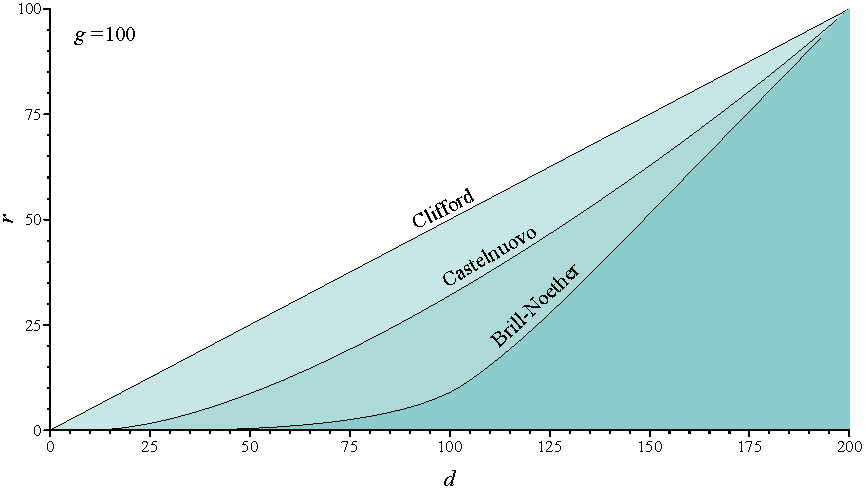
\includegraphics[width=0.9\hsize]{main/Fig11-1-new}
\caption{For smooth curves of genus 100,
these are bounds on $(d,r)$ for all linear series (Clifford),
birationally very ample series (Castelnuovo), and all linear series
on general curves (Brill--Noether).
}
\label{Clifford-Castelnuovo-BrillNoether comparison}
\end{figure}

Gathering the inequalities, and putting them all in terms of lower bounds
on $d$ given $g, r$,
we get
$$
\eqalign{
\noalign{\vskip3pt}
 d &\geq \min\{r+g, 2r\}&\quad& \hbox{ (by the Riemann--Roch and Clifford
 theorems)},\cr
\noalign{\vskip1pt}
 d &\geq \sqrt{(2r-2)\smash{g}}&& \hbox{ (by an approximation to the Castelnuovo
 theorem)},\cr
 d &\geq r+g-\frac{g}{r+1}&& \hbox{ (for a general curve)}.
}
$$

In the following sections, we'll explain the heuristic argument that
led Brill and Noether to the statement of Theorem~\ref{basic BN} and
discuss some refinements.   In Chapter~\ref{InflectionsChapter} we'll
give a proof based on the study
of inflections and on families of Jacobians.

The case $r=1$ is already interesting:

\begin{corollary}\label{gonality bound}
If $C$ is any curve of genus $g$, then $C$ admits a map  to $\PP^1$
of degree $d$ for some $d \leq \bigl\lceil \frac{g+2}{2}\bigr\rceil$.
\end{corollary}

Thus any curve of genus 2 is hyperelliptic, any curve of genus 3 or
4 is either hyperelliptic or trigonal  (admits a 3-1 map to $\PP^1$),
and so on. We have already verified this assertion in genus $g \leq 5$
by analyzing the geometry of the canonical map; for higher genera,
though, this is not feasible.

Note also that this is exactly the converse to Corollary~\ref{branched
cover BN} of Chapter~\ref{ModuliChapter}.


\subsection{A Brill--Noether inequality}\label{BN by divisors}
%12.2.1

The proof of the Brill--Noether theorem starts with a dimension
estimate that was first carried out in
\cite{Brill-NoetherOriginal}. The estimate provides an inequality on
the dimension of the variety $W^r_d$, and the assertion of the theorem
is that this is sharp for a general curve.

%From Kleiman-Laksov:  For r= 1, the matter is treated in section 4
%of Riemann's " Theorie der Abel'schen Functionen" [11] (1857) and in
%lecture 31 of Hensel-Landsberg(1902) 1; the general case is treated
%in Brill--Noether [1](1874) and in lecture 57 and appendix G of Severi
%[13].(1921)

Let $C$ be a smooth projective curve of genus $g$, and $D = p_1 + \dots
+ p_d$ a divisor on $C$. Assume for simplicity that  the points $p_i$
are distinct; the same argument  can be carried out in general, but
requires more complicated notation.

When does the divisor $D$ move in an $r$-dimensional linear series? By
the
Riemann--Roch theorem
\index{Riemann--Roch theorem}%
$h^0(D) \geq r+1$ if and only~if the vector
space $H^0(K-D)$ of 1-forms vanishing on $D$ has dimension at least
$g-d+r$\emdash that is, if and only~if the  evaluation map
$$
H^0(K) \to H^0(K|_D) = \tsty\bigoplus k_{p_i}
$$
has rank at most $d-r$.

We can represent this map by a $g \times d$ matrix. Choose a basis
$\omega_1,\dots,\omega_g$ for the space $H^0(K)$ of 1-forms on $C$;
choose an analytic open neighborhood $U_j$ of each point $p_j \in D$
and choose a local coordinate $z_j$ in $U_j$ around each point $p_j$,
and write
$$
\omega_i = f_{i,j}(z_j)\,dz_j
$$
in $U_j$. We  have $r(D) \geq r$ if and only~if the  matrix-valued
function
$$
A(z_1,\dots,z_d) =
\begin{pmatrix}
f_{1,1}(z_1) & f_{2,1}(z_1) & \dots & f_{g,1}(z_1) \\
f_{1,2}(z_2) & f_{2,2}(z_2) & \dots & f_{g,2}(z_2) \\
\vdots & \vdots &  & \vdots \\
f_{1,d}(z_d) & f_{2,d}(z_d) & \dots & f_{g,d} (z_d)
\end{pmatrix}
$$
has rank $d-r$ or less at $(z_1,\dots,z_d) = (0,\dots,0)$.


In the space $M_{d,g}$ of $d \times g$ matrices, the subset of matrices
of rank $d-r$ or less has codimension $r(g-d+r)$
\cite[Exercise 10.9]{Eisenbud1995}.
It follows
that if  an effective divisor $D$ of degree $d$ with $h^0(D) \geq r+1$
exists, then in a neighborhood of the point $D \in C_d$ the locus
$C^r_d$ of such divisors must have dimension at least $d - r(g-d+r)$,
with equality if the map $A$ is dimensionally transverse to the locus
in $M_{d,g}$ of matrices of rank at most $d-r$. Since a general fiber
\index{C@$C^r_d$}%
\index{W@$W^r_d$}%
of the map $\mu :
C^r_d
 \to
W^r_d
(C)$ has dimension $r$, it follows that
$$
\dim W^r_d(C) \geq d - r(g-d+r) - r = g - (r+1)(g-d+r)
$$
and this is exactly the  Brill--Noether (in)equality. We will give a proof
of the Brill--Noether theorem in Chapter~\ref{BrillNoetherproofChapter}.


\subsection{Refinements of the Brill--Noether theorem}

Theorem~\ref{basic BN} suggests a slew of questions, both about the
geometry of the schemes $W^r_d(C)$ parametrizing linear series on a
general curve $C$ (are they irreducible? what are their singular
loci?), and about the geometry of the linear systems themselves (do
they give embeddings? what's the Hilbert function of the image?). This
is an active area of research. Here is some of what is currently
known, starting with results about the geometry of $W^r_d(C)$:

\begin{theorem}\label{Wrd omnibus}
Let $C$ be a general curve of genus $g$,
and set
$$\rho = g - (r+1)(g-d+r).$$
Assume that $d \leq g+r$. Then:
\begin{enumerate}

\item $\dim(W^r_d(C)) = \rho$
{\rm\cite{Griffiths-Harris-BN}}.
\label{GH}

\item\label{sing wrd} The singular locus of $W^r_d(C)$ is exactly
$W^{r+1}_d(C)$
{\rm\cite{Gieseker-Petri,Lazarsfeld-Petri}}.
\label{irr wrd}

\item If $\rho > 0$ then $W^r_d(C)$ is irreducible
\index{Gieseker, David}%
\index{Fulton, William}%
\index{Lazarsfeld, Robert}%
{\rm\cite{MR611386}}.

\item\label{rho=0} If $\rho = 0$ then $W^r_d(C)$ consists of a finite
set of  points of cardinality
$$
\#W^r_d(C) = g! \prod_{\alpha=0}^r \frac{\alpha!}{(g-d+r+\alpha)!}
$$
and the monodromy of the generically finite covering of  $M_g$ by the
universal family
$\cW^r_d$ of $W^r_d$s is transitive
{\rm\cite{zbMATH04014883}}.

\item\label{Petri} If  $\sL$ is an invertible sheaf on $C$, then the
multiplication map
$$
m : H^0(L) \otimes H^0(\omega_C\otimes L^{-1}) \to H^0(\omega_C)
$$
is injective, and the Zariski tangent space to the scheme $W^r_d(C)$
at the point $L$, as a subspace
of the tangent space $T_L\pic_d(C) = H^0(\omega_C)^*` `$, is the
annihilator of the image of $m$
or, equivalently, the kernel of the dual of $m$
{\rm\cite{Gieseker-Petri}}.
\end{enumerate}
\end{theorem}

\begin{corollary}\label{2L nonspecial}
If $C$ is a general curve and $\sL$ is a general point of $W^r_d(C)$
with $r\geq 2$,
 then $\sL^m$ is nonspecial for all $m \geq 2$.
\index{nonspecial}%
\end{corollary}

\begin{proof}
If $\sL^m$ were special\emdash that is, if $\omega_C\otimes \sL^{-m}
= E$ were effective\emdash then we would have an inclusion $H^0(\sL) =
H^0(\omega_C\otimes \sL^{-m+1}(-E)) \hookrightarrow H^0(\omega_C\otimes
\sL^{-m+1})$. By part~\ref{Petri} of Theorem~\ref{Wrd omnibus}, the map
 $$
m : H^0(\sL^{m-1}) \otimes H^0(\omega_C\otimes \sL^{-m+1}) \to
H^0(\omega_C)
$$
is injective, so the map
$$
H^0(\sL^{m-1}) \otimes H^0(\sL) \subset H^0(\sL^{m-1}) \otimes
H^0(\omega_C\otimes \sL^{-m+1})
$$
obtained by restriction would likewise be injective.
However if $\sigma, \tau \in H^0(\sL)$ are two linearly independent
sections, then $\sigma^{m-1} \otimes \tau - \sigma^{m-2}\tau \otimes
\sigma$ lies in the kernel, contradicting the specialness of $\sL^m` `$.
\end{proof}
\begin{remark}
 As a special case of part~\ref{rho=0} of the theorem we see that
 the number of $g^{1}_{d}$s
 in the case $\rho=0$
(that is to say,
$g=2d-2$) is the
Catalan number
\index{Catalan number}%
 $C_{d-1}\colonequals  \tbinom{2d}{d}\big/ d$.

We have already seen this in the first two cases: in genus 2, it says
the canonical series $|K|$ is the unique $g^1_2$ on a curve of genus 2,
and in the case of genus 4 we have already seen  that there are exactly
two $g^1_3$s on a general curve of genus 4. In genus 6, it says that
a general curve of genus 6 has 5 $g^1_4$s; we'll describe these in
Section~\ref{general genus 6} below.
\end{remark}

\begin{remark}
Parts~(\ref{Petri}) and (\ref{GH}) of the theorem imply part~(\ref{sing wrd}).
\cite[Section IV.4]{ACGH} shows that at a point $\sL  \in W^r_d(C)
\setminus W^{r+1}_d(C)$, the tangent space to $W^r_d$ at the point $\sL $
is the annihilator
in $(H^0(\omega_C))^*$ of the image of $\mu$; given that $\mu$ is
injective, we can compare dimensions and deduce that $W^r_d$ is smooth
at $\sL $.
\end{remark}

\begin{remark}
For any curve $C$, there exists a scheme $G^r_d(C)$ parametrizing
linear series of degree $d$ and dimension $r$; that is, in set-theoretic
terms,
$$
G^r_d(C) = \left\{ (\sL , V) \mid \sL  \in Pic_d(C), \text{ and }
V \subset H^0(\sL ) \text{ with } \dim V = r+1 \right\}.
$$
$G^r_d(C)$ maps to $W^r_d(C)$; the map is an isomorphism over the open
subset $W^r_d(C) \setminus W^{r+1}_d(C)$ and has positive-dimensional
fibers over $W^{r+1}_d(C)$. It was conjectured
by Petri and proven in \cite{Gieseker-Petri} that for a general curve
the scheme $G^r_d(C)$ is smooth for any $d$ and $r$.
\end{remark}


Recall that  in theorems~\ref{g+1 theorem}, \ref{g+2 theorem}, \ref{g+3
theorem} we proved that
general invertible sheaves of degrees $g+1$, $g+2$ and $g+3$ on any curve
give the nicest possible maps to (respectively) $\PP^1, \PP^2$ and
$\PP^3$. These
linear series, being general of degree $\geq g$, are  nonspecial and
have respectively
2, 3, or 4-dimensional spaces of sections. The following result shows
that something
similar is true on a general curve for general linear series with 2,3,
or 4-dimensional
spaces of sections, though they may have degrees much less than $g+1,
g+2, g+3$:

\begin{npt}
\begin{theorem}[{{\cite[Proposition 5.4]{Eisenbud-Harris83}}}]
\label{grd omnibus}
Let $C$ be a general curve of genus $g$, and suppose that
$|D|$ is a general $g^r_d$ on $C$.

 \begin{enumerate}
\item If $r \geq 3$ then $D$ is very ample; that is, the map $\phi_D :
C \to \PP^r$   embeds $C$ in $\PP^r` `$;
\item If $r=2$ the map $\phi_D : C \to \PP^2$ gives a birational embedding
of $C$ as a nodal plane curve; and
\item If $r=1$, the map $\phi_D : C \to \PP^1$ expresses $C$ as a simply
branched cover of $\PP^1` `$.
\end{enumerate}
\end{theorem}
\end{npt}

In case $\rho = 0$\emdash so that there are a finite number of $g^r_d$s
on a general curve $C$\emdash these statements hold for \emph{all}
the $g^r_d$s on $C$.

In the course of investigating embeddings of a curve $C\subset \PP^n$
we have again and again
asked about the ranks of the maps $H^0(\sO_{\PP^n}(d)) \to
H^0(\sO_C(d))$. In the case of
a general curve, the following theorem of
E. Larson
\index{Larson, Eric}%
gives a
comprehensive answer,
which is the same as giving
 the Hilbert function of the image curve:

\begin{theorem}[maximal rank theorem \cite{Larson}]\label{maximal rank}
If $C$ is a general curve of genus $g$ and $\sL  \in W^r_d(C)$ is a
\index{maximal rank theorem}%
general point, then for each $m > 0$ the multiplication map
$$
\rho_m : \Sym^m H^0(\sL ) \to H^0(\sL ^m)
$$
has maximal rank; that is, it is injective if $\tbinom{m+r}{r} \leq
h^0(\sL ^m)$ and surjective if $\tbinom{m+r}{r} \geq h^0(\sL ^m)$.
\end{theorem}


If $\sL\in W^r_d(C)$ is a general point, then Corollary~\ref{2L nonspecial}
shows that $h^0(\sL ^m) = md-g+1$ for all $m \geq 2$,
and this allows us to compute the Hilbert function of a general embedding
as a curve
of degree $d$ as
 $$
 h_C(m) = \min\left(\mbinom{m+r}{r},\ md-g+1\right).
 $$

A key step in Larson's proof is an interpolation theorem \cite{MR3908670},
later extended
as follows:
\index{Larson, Eric}%
\index{Vogt, Isabel}%

\begin{npt}
\begin{theorem}[\cite{MR4653767}]\label{Larson-Vogt}
Let $d, g$ and $r$
be nonnegative integers with $\rho(d, g, r) \geq 0$. There is a general
curve of degree $d$ and genus $g$ through $n$ general
points in $\PP^r$
if and only~if
$$
(r-1)n \leq (r + 1)@d-(r-3)(g-1)
$$
except in the four cases $(d, g, r) = (5, 2, 3)$,
$(6, 4, 3)$, $(7, 2, 5)$ and $(10, 6, 5)$.
 \end{theorem}
\end{npt}

There is a possible extension of the maximal rank theorem. If $C
\subset \PP^r$ is a general curve embedded by a general linear series,
the maximal rank theorem tells us the dimension of the $m$-th graded
piece of the ideal of $C$, for any $m$: this is just the dimension of
the kernel of $\rho_m$. But it doesn't tell us the degrees of
\index{generators of homogeneous ideal}%
generators of the homogeneous ideal of $C$. For example, if $m_0$ is
the smallest $m$ for which $I(C)_m \neq 0$, or numerically the
smallest $m$ such that $\tbinom{m+r}{r} > md-g+1$, we can ask: is the
homogeneous ideal $I(C)$ generated by $I(C)_{m_0}$? This can't always
be the case, since
there are examples where the  smallest nonzero graded piece of $I(C)$ has
dimension 1. But one might conjecture that $I(C)$ is always be generated
by its graded pieces of degrees $m$ and $m+1$; this is an open problem.

To answer this, given that we know the dimensions of $I(C)_m$ for
every~$m$, we would need to know the ranks of the multiplication
maps
$$
\sigma_m : I(C)_m \otimes H^0(\cO_{\PP^r}(1)) \to I(C)_{m+1}
$$
for each $m$. In particular, we may conjecture that \emph{the maps
$\sigma$ have maximal rank}; if this were true we could deduce the
\index{maximal rank}%
degrees of a minimal set of generators for the homogeneous ideal $I(C)$.

Another recent strand of work on Brill--Noether theory was developed in
the thesis
\cite{HLarson} and in \cite{arXiv:2008.10765}, providing  analogues of
many of the parts of the classical Brill--Noether theorem
\index{Brill--Noether theory|)}%
\index{Brill--Noether theorem!for curves of give gonality}%
\index{gonality}%
for general curves of given gonality in the cases $\rho\geq 0$.

There are many remaining questions! One is the question of \emph{secant
planes}: a naive dimension count would suggest that an irreducible,
nondegenerate curve $C \subset \PP^r$ should have an $s$-secant $t$-plane
if and only~if $s(r-t-1) \leq (t+1)(r-t)$
(for example a curve $C \subset \PP^3$ has 4-secant lines, but no
5-secant lines; see Exercise~\ref{out of place}). 
Is this true for a general curve embedded in $\PP^r$
by a general linear series?

\section{Linear series on curves of genus 6}
\label{genus 6 section}\label{general genus 6}

We have seen in our analysis of curves of genus up to 5 that curves of the
same genus can look quite different from the point of view of the linear
series they possess: the existence of $g^r_d$s,  the geometry of the
schemes $W^r_d(C)$ parametrizing them, and the geometry of the associated
maps to projective space, can look quite different on different curves.

The variety of possible behaviors has increased modestly with the
genus. Genus 6 is a tipping point: we could still enumerate all the
possible behaviors of the schemes $W^r_d(C)$\emdash as distinguished
by the number of components, dimension and singularities of the various
schemes $W^r_d(C)$, and the geometry of the associated maps\emdash but
it's quite a long list, and we will actually study just a few cases. For
genus 7 and higher a full analysis has probably never been carried out.

In lower genus we tacitly verified the statements of the Brill--Noether
theorem from our descriptions of the canonical models. In genus 6, by
contrast, we cannot  deduce the Brill--Noether theorem from studying
the geometry of the canonical curve\emdash though we can easily see that
a canonical curve $C \subset \PP^5$ of genus 6 lies on a 6-dimensional
vector space of quadrics, that doesn't tell us much about its geometry.

Instead we will appeal directly to the Brill--Noether theorems. Here is
a summary of what we will use:

\begin{theorem}\label{BN consequences}
Every smooth curve $C$ of genus 6 has at least one $g^{2}_{6}$. If $C$
is general, then
$W^{2}_{6}(C)$ and $W^{1}_{4}(C)$ each consist of 5 reduced points,
while $W^{2}_{5} = W^{1}_{3} = \emptyset$.  Less formally, C has
precisely 5 $g^{2}_{6}$s and 5 $g^{1}_{4}$s, but no $g^{2}_{5}$s and
no $g^{1}_{3}$s. The image of the map associated to each $g^{2}_{6}$
is a nodal plane curve and its nodes are in linearly general position,
that is, no three are collinear.
\end{theorem}

All these assertions except for the linear general position of the nodes
follow immediately from
Theorem~\ref{basic BN} and
Theorem~\ref{Wrd omnibus}; we will deduce the linear general position
of the nodes from the relationship of the different
linear series on a general curve that are given by these theorems.

%\subsection{Linear series on general curves of genus 6}\label{general genus 6}
\subsection{General curves of genus 6}
\emph{We suppose for the rest of this section that $C$ is a general
smooth curve of genus 6.}

By Theorem~\ref{BN consequences} we can map $C$ birationally to a plane
sextic $C_0$ with only nodes as singularities. Since a plane sextic has
arithmetic genus $\tbinom{6-1}{2} = 10$, the curve $C_{0}$
must have exactly 4 nodes.

Once we have exhibited one birational map of $C$ to a plane sextic with
4 nodes, we can describe all five $g^2_6$s and all five $g^1_4$s in terms
of this plane model. For example, composing a $g^1_6$ corresponding to $f:
C\to \PP^1$ with the projections from the 4 nodes gives four $g^1_4$s. To
see the
fifth
$g^{1}_{4}$ we introduce some terminology:

Suppose $f : X \to S$ is a regular map from any smooth curve $X$ to a
surface $S$. If $\sL $ is a line bundle on $S$ and $V \subset H^0(\sL
)$ a vector space of sections, we can associate to them a linear system
on $X$ by taking the pullback linear system $f^*V \subset H^0(f^*\sL )$
on $X$ and subtracting the basepoints; this is called the
\emph{linear series cut out on $X$ by $V$}.
\index{linear series!cut out on $X$ by $V$}%

\begin{figure}[b]
\hskip0pt
\raise3pt\hbox{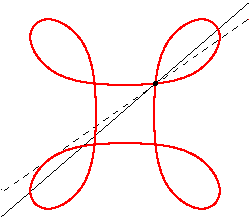
\includegraphics[width=0.36\hsize]{main/Fig11-2-new}\quad}
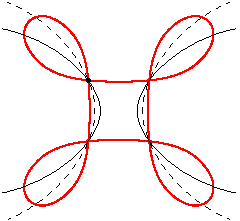
\includegraphics[width=0.34\hsize]{main/Fig11-3-new}
\caption{Left: A $g^1_4$ as (left)
the projection from a node of a plane sextic
and (right)
a pencil of conics through the four nodes of a
plane sextic.
}
\label{plane sextic 1}
\end{figure}

To see the $g^{1}_{4}$s on $C$ in this way,  suppose again that $C$ is a
general curve of genus 6 as above and $f : C \to \PP^2$ is a birational
map onto a sextic curve $C_0$ with four nodes; let $p \in C_0$ be one of
the nodes and consider the linear system $(\cO_{\PP^2}(1),V)$ of lines
in $\PP^2$ through $p$. The pullback $f^*\cO_{\PP^2}(1)$ of course has
degree 6, but the pullback linear series $f^*V$ has two basepoints,
at the points $q, r \in C$ lying over $p$. The linear series cut on $C$
by $V$ is thus a $g^1_4$; see Figure~\ref{plane sextic 1}, left.

To produce the fifth $g^1_4$, consider the linear series cut on
$C$ by conic plane curves passing through all four nodes of $C_0$
(Figure~\ref{plane sextic 1}, right).  There is a pencil of such conics, and
the pullback $f^*\cO_{\PP^2}(2)$ has degree 12.
If the nodes are linearly independent then the pullback series has eight
basepoints; thus we arrive at another $g^1_4$ on $C$.  Not all the nodes
can be contained in a line, since then, by B\'ezout's theorem, the line
\index{B\'ezout's theorem}%
would be a component of $C_0$. Thus if the nodes are linearly dependent,
then exactly 3 lie on a line
so the linear series cut by the conics containing the nodes coincides
with the projection from the
fourth
node.
This would represent a nonreduced point of the scheme $W^1_4(C)$,
the subject of Exercise~\ref{nonreduced Wrd} below. Thus the nodes
are independent.

For another example, consider the linear system cut on $C$ by cubics
passing through all four nodes. This has degree $3\cdot 6 - 8 = 10$
and dimension 6. It follows that this is the
complete canonical series
\index{complete canonical series}%
on $C$. (In Chapter~\ref{PlaneCurvesChapter} we will see directly that
this is the case.)

Given the degree six map $f : C \to C_0 \subset \PP^2$ corresponding
to one $g^2_6$ we can use the fact that the five $g^2_6$s on $C$ are
residual to the five $g^1_4$s in the canonical series to construct the
other four $g^2_6$s: they are cut out on $C$ by the linear system of plane
conics passing through three of the four nodes of $C_0$  Equivalently,
their images are the curves obtained from $C_{0}$ by the quadratic
transformation
of $\PP^{2}$ centered at 3 of the 4 nodes, which blows up these 3 nodes
and blows down the three lines
 joining them (Figure~\ref{plane sextics 3}).

 In previous chapters we have seen that in genus $\leq 5$ a general
 canonical curve is  a complete intersection, but this fails for a
\index{complete intersection}%
 canonical curve $C$ of genus 6. There is a 21-dimensional vector space of
quadratic forms on $\PP^5` `$, and $h^0(\sO_C(2)) = 2(2g-2)-g+1 = 15$,
so $C$ lies on at least 6 quadrics, and we will show that its ideal sheaf
is generated by exactly 6 quadrics. Since $6>\codim C$, the canonical
curve of genus 6 is not a complete intersection. However, such curves
lie on a quintic del Pezzo surface, which may be described as follows.
\index{del Pezzo surface}%
\index{del Pezzo surface!quintic|(}%

%There is a further consequence of this description: the four nodes of
%$C_0$ are in linear general position; that is, no three are collinear.
%By parts~(\ref{rho=0}) and~\ref{Petri} of Theorem~\ref{Wrd omnibus}, $C$
%must have 5 distinct $g^1_4$s, and if three of the four nodes of $C_0$
%were collinear, the $g^1_4$ cut on $C$ by lines through the fourth node
%would coincide with the $g^1_4$ cut on $C$ by conics through all four.

\begin{figure}
\centerline {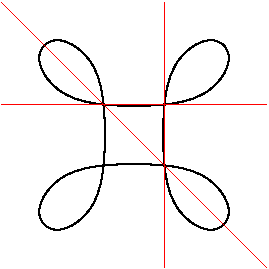
\includegraphics[height=1.5in,trim=10 10 10 10,clip]{main/Fig11-4-new}}
\caption{A sextic with 4 nodes and the fundamental triangle of the
quadratic transformation giving
a different $g^{2}_{6}$.}
\label{plane sextics 3}
\end{figure}


\subsection{Del Pezzo surfaces}\label{Del Pezzo sketch}
%12.3.2

We  met the del Pezzo surface of degree 5 in Section~\ref{Genus 1 quintics
in P4}.
We briefly sketch, without proofs, a little of the
 rich classical theory of del Pezzo surfaces in general. The basics are
 well treated in \cite[pp.~45--50]{Beauville}; for more, see the
beautiful book \cite{Manin}, which also goes into some of the arithmetic
\index{Manin, Yuri I.}%
\index{Beauville, Arnaud}%
theory. We will use only the case of the del Pezzo surface of degree 4,
which lies in $\PP^{5}$

By definition,
a \emph{del Pezzo} surface is a smooth surface embedded in $\PP^n$  by
its complete anticanonical series $-K_S$. These exist only for $3\leq
n\leq 9$. The best-known example is a smooth cubic surface in $\PP^3``$.
That it is a del Pezzo surface follows from the adjunction formula.

A del Pezzo surface in $\PP^n$ has degree $n$, and is isomorphic to the
blow-up of $\PP^2$ at $9-n$ points of which no 3 lie on a line and no
6 lie on a conic, embedded by the linear series on $\PP^2$
consisting of the cubics passing through the $9-n$ points\emdash except
when $n=8$, in which case the
linear series of curves of type $(2,2)$ on $\PP^1\times \PP^1$ provides
another example.

Comparing the linear series  of cubic forms containing $p_1,\dots,p_4$
with the linear series  of sextic forms vanishing to order 2 at
$p_1,\dots,p_4$, we see that a quintic del Pezzo surface $S \subset \PP^5$
lies on at least $5$ quadrics. In fact, its homogeneous ideal is generated
by exactly 5 quadrics.

A quintic del Pezzo surface $S \subset \PP^5$ contains exactly 10 lines,
which (in terms of the description of $S$ as the blow up of $\PP^2$ at
four points $p_1,\dots,p_4 \in \PP^2$) are the 4 exceptional divisors
and the 6 proper transforms of the lines joining the $p_i$ pairwise. The
configuration of these lines is shown in Figure~\ref{dual graph of the
configuration of 10 lines on a quintic del Pezzo surface}.
It is the intersection of a $\PP^5$ with the Grassmannian $G(2,5)
\subset \PP^9` `$, and correspondingly the five quadrics containing $S$
can be realized as the Pfaffians of a  $5\times 5$ skew-symmetric matrix
of linear forms on $\PP^5` `$.

\begin{figure}
\centerline {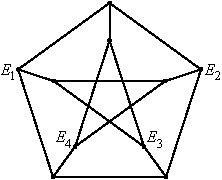
\includegraphics[height=1.4in]{main/Fig11-5}}
\caption{Dual graph of the configuration of 10 lines on a quintic del
Pezzo surface, the plane blown up
at 4 points showing 4 pairwise disjoint exceptional divisors.}
\label{dual graph of the configuration of 10 lines on a quintic del
Pezzo surface}
\end{figure}

There is also a notion of a \emph{weak del Pezzo}
\index{weak del Pezzo}%
surface; this is a
smooth surface whose
anticanonical bundle
\index{anticanonical bundle}%
 is
nef but not necessarily ample.
\index{nef but not necessarily ample}%
We get such a surface if we blow up $\PP^2$ at a configuration
of points of which three are collinear; in this circumstance the
anticanonical bundle on the blow-up $S$ has degree 0 on the proper
transform of the line containing the three points, and this proper
transform is correspondingly collapsed to a rational double point of the
image $\phi_{-K}(S)$. In general, the description of del Pezzo surfaces
as blow-ups of the plane extends to the case of weak del Pezzos.



\subsection{The canonical image of a general curve of genus 6}

Using the Brill--Noether theorem, we have seen that a general curve $C$
of genus 6 is the normalization of a plane sextic $C_0$ with four nodes,
and that the canonical series on $C$ is cut out by cubics in the plane
passing through the four nodes. Thus the canonical model lies on the
surface $S \subset \PP^5$ that is the image of the plane under the
(rational) map given by cubics through these four points, which we now
recognize as a quintic del Pezzo surface.

\begin{theorem}
A general canonical curve $C$ of genus 6 is the intersection of a quintic
del Pezzo surface and a quadric.
\end{theorem}

\begin{proof}
We have seen that $C \subset \PP^5$ lies on a quintic del Pezzo surface
\index{del Pezzo surface!quintic|)}%
$S \subset \PP^5` `$. The surface is cut out by 5 quadrics, and we know
that $C$ lies on 6 independent quadrics,
so $C$ is contained in the complete intersection of $S$ with a
quadric. Since this scheme has degree 10, which is the degree of $C$,
they are equal.
\end{proof}

For corresponding theorems for general curves with $g=7,8,9$ see
\cite{Mukai1}, \cite{Mukai2}, and \cite{Mukai3}.


\section{Other curves of genus 6}

From Theorem~\ref{BN consequences} we know that every curve $C$ of genus
6 has  a $g^{2}_{6}$. For a general curve the corresponding morphism
$\phi_{D}$ maps $C$ birationally onto a plane sextic with 4 nodes and
exactly 5 $g^{1}_{4}$s.
In this  section we will analyze some of the other curves of genus 6,
starting with the question  ``what could go wrong?''
with the birational map to $\PP^2` `$.

Since we already have a complete picture in the hyperelliptic case, we'll
assume that $C$ is nonhyperelliptic. Clifford's theorem then rules out
the existence of a $g^3_6$ so  the $g^2_6$ is a complete linear series
$|D|$ for some divisor $D$ of degree 6.

Further analysis can be divided as follows:
\smallbreak
\noindent\underline{Case 1}:
$C$ is not
trigonal.
\index{trigonal}%
\begin{enumerate}\def\theenumi{\alph{enumi}}
 \item $|D|$ has a basepoint; the canonical image of $C$ lies on the
 Veronese surface.
\item $\phi_{D}$ maps $C$
two-to-one
\index{2-fold cover}%
onto a cubic $E \subset \PP^2$ of
genus 1; the canonical image is the
complete intersection
\index{complete intersection}%
of a quadric
and the
cone over the elliptic quintic
\index{cone!over elliptic quintic}%
\index{quintic!elliptic}%
$E\subset \PP^{4}$.
\item $\phi_{D}$ is birational onto a plane sextic with no triple point.
 \end{enumerate}
\noindent\underline{Case 2}:
$C$ is trigonal. The canonical image lies on a
rational normal scroll $S(a,4-a)$; see Chapter~\ref{ScrollsChapter}.
In this case $|D|$ is basepoint free and $\phi_{D}$  either maps $C$
three to one onto a conic
 or birationally onto a
sextic with a triple point.
\index{3-fold cover!of conic}%
\index{sextic!with triple point}%
\index{triple point!on sextic}%
\smallbreak

In the rest of this section we will examine cases 1(a) and 1(b). Case 2 can
be further divided by the value of $a$.
Case 1(c) may be divided into many parts according to the various
configurations
of double points of the plane sextic, which may be nodes, cusps, tacnodes
or higher-order double points,  corresponding to various possible
schemes $W^{1}_{4}$.

The analysis of the other cases is lengthy, but largely accessible with
the tools we've introduced.


\subsection*{$|D|$ has a basepoint}
%\label{g26 has a basepoint}

Clifford's theorem shows that a nonhyperelliptic curve of genus 6 cannot
have a $g^2_4$, so
$|D|$ has exactly one basepoint, and when we subtract the basepoint we
get a basepoint-free $g^2_5$.

If $C \to C_0 \subset \PP^r$ is the map given by a basepoint free $g^r_d$,
the degree $d$ of the linear series is the degree of the image curve $C_0$
times the degree of the map $C \to C_0$. Since 5 is prime, the associated
map $\phi_D : C \to \PP^2$ is birational onto a quintic curve. Moreover,
since
\index{plane quintic}%
plane quintic
 curves have
arithmetic genus 6,
\index{arithmetic genus 6}%
the image $\phi_D(C)$
is smooth; thus $C$ is isomorphic to a smooth plane quintic.

This allows us to describe the other special linear series on $C$. By
the adjunction formula, the canonical series $|K_C|$ is cut on $C$
by conics in the plane.

The plane $\PP^2$ is embedded by the complete linear series of quadrics
as the
{Veronese surface in $\PP^5``$,
\index{Veronese surface in $\PP^5$}%
of $C$ is cut out by quadrics, the canonical model of $C$
lies on this surface, and the canonical ideal is generated by the
6-dimensional family of quadrics containing the Veronese surface\emdash
the $2\times 2$ minors of the generic symmetric $3\times 3$ matrix
corresponding to the multiplication map
$$
H^{0}(\sO_{\PP^{2}}(1)) \otimes H^{0}(\sO_{\PP^{2}}(1)) \to
H^{0}(\sO_{\PP^{2}}(2))
$$
as explained in Proposition~\ref{some equations}-- together with a
3-dimensional family of cubics,  the image of the 3 dimensional family
of forms of degree 6 that are multiples of the quintic form defining $C$
in $\PP^2` `$.

As we showed in Chapter~\ref{3b}, the $g^1_4$s on $C$ are exactly the
projections from points of $C$, so $W^1_4(C)\cong C$, and there are no
$g^{1}_{3}$s.


\subsection*{$C$ is not trigonal and the image of
\texorpdfstring{$\phi_{D}$}{phi(D)} is two-to-one onto a  plane curve
of degree 3.}

The cubic curve $E$ is smooth since otherwise it would have geometric
genus 0 and $C$ would be  hyperelliptic. Thus $C$ is a double cover of
a smooth curve of genus 1; we say that $C$ is \emph{bielliptic}.
\index{bielliptic}%

In this case the canonical divisor class $K_C$ is the pullback of
an invertible sheaf $\cO_E(F)$ for some divisor class of degree 5 on
$E$. But it is not the case that the canonical series $|K_C|$ is the
pullback of the linear series $|\cO_E(F)|$: by the Riemann--Roch theorem,
the latter has dimension 4, rather than 5. Indeed, if we recall that
the target of the canonical map $\phi_K : C \to \PP^5$ is the projective
space $\PP H^0(K_C)$, there is be a point $X \in \PP^5$ corresponding to
the hyperplane $\pi^*H^0(F) \hookrightarrow H^0(K_C)$, and projection
of the canonical curve from this point maps $C$ 2-to-1 onto the image
$\phi_F(E) \subset \PP^4` `$. In other words, the canonical model of $C$
lies on a cone $S = \overline{X, E}$ over an elliptic normal quintic
curve $E \subset \PP^4` `$.

As we saw in Chapter~\ref{3b}, the quintic curve $\phi_F(E) \subset \PP^4$
lies on 5 quadrics, as does the cone $S \subset \PP^5$ over it. Thus
there is a quadric $Q \subset \PP^5$ containing $C$ but not containing
$S$. B\'ezout's theorem shows that in this case, the canonical model of
a bielliptic curve of genus 6 is the intersection of the cone over an
elliptic quintic curve with a quadric.

\section{Exercises}

\begin{exercise}
\label{out of place}
We saw in Chapter~\ref{JacobianChapter} that if $C$ is any curve of genus
$g$ and $D$ a general divisor of degree $g+3$ on $C$, then $\phi_D :
C \hookrightarrow \PP^3$ is an embedding. Using the Brill--Noether
theorem, show that if $C$ is general then the image curve in $\PP^3$
has no 5-secant lines.
\end{exercise}

\begin{exercise}
Let $C$ be a bielliptic curve of genus 6; that is, a double cover of a
\index{bielliptic}%
smooth projective curve $E$ of genus 1.
\begin{enumerate}
\item Show that $C$ cannot be hyperelliptic (going forward, we will
identify $C$ with its canonical image in $\PP^5$).
\item Let $F$ an invertible sheaf of degree 5 on $E$ and $\phi_F(E)
\subset \PP^4$ the corresponding elliptic normal quintic curve. Show that
$\phi_F(E)$ lies on 5 quadrics, as does the cone $S \subset \PP^5$ over it.
\tohint{12-02}
\item Deduce that there is a quadric $Q \subset \PP^5$ containing $C$
but not containing $S$. Now invoke B\'ezout's theorem to deduce that in
this case, the canonical model of a bielliptic curve of genus 6 is the
intersection of the cone over an elliptic quintic curve with a quadric.
\end{enumerate}
\end{exercise}

\begin{exercise}
Use the preceding exercise to show that if $C$ is a bielliptic curve of
genus 6, a 2-sheeted cover of an elliptic curve $E$, then every $g^1_4$
on $C$ is the pullback of a $g^1_2$ on $E$, and likewise  every $g^2_6$
on $C$ is the pullback of a $g^2_3$ on $E$. Deduce that in this case,
$W^1_4(C)$ and $W^2_6(C)$ are each isomorphic to $E$.
\tohint{12-03}
\end{exercise}

\begin{exercise}
Let $C$ be a trigonal curve of genus 6 with $g^1_3$ $|E|$, and $p \in C$
a general point. Show that the linear series $|K_C - E-p|$ is a $g^2_6$,
and that the corresponding map $C \to \PP^2$ maps $C$ birationally onto
a plane sextic curve with a triple point.
\end{exercise}

\begin{exercise}\label{plane models}
Let $C$ be the normalization of a plane sextic $C_0$ with four nodes,
three of which are collinear. Show that by choosing a different $g^2_6$
on $C$, we can express it as the normalization of a plane sextic with
two nodes and a tacnode.
\tohint{12-05}
\end{exercise}

\begin{exercise}
Show that if $C$ is the normalization of a plane sextic $C_0$ with only
double points, then $W^1_4(C) \cong W^2_6(C)$ is zero-dimensional (so
in particular this case does not overlap with any of the previous cases)
\end{exercise}

\begin{exercise}
Find an example of a curve $C$ of genus 6 such that $W^1_4(C)$ consists
of one point of degree 5. Bonus points for showing that in this case
the scheme $W^1_4(C) \cong \Spec \CC[\epsilon]/(\epsilon^5)$.
\tohint{12-07}
\end{exercise}

\begin{exercise}
Show that if $C$ is a smooth plane quintic, then the $g^2_6$s on $C$
all have a basepoint; that is, they are all of the form $|K_C| + p$
for $p \in C$.

Furthermore, the canonical model of $C$ will lie on a quadratic Veronese
surface $S$; and the six
quadrics containing the canonical curve $C$ are the six quadrics
containing $S$.
In particular, the intersection of the quadrics containing
$C$ will be $S$, so
the ideal of $C$ requires generators of degree $>2$.
\end{exercise}

\begin{exercise}\label{nonreduced Wrd}
Show that if the nodes of the curve $C_0$ are in linear general
position\emdash that is, no three
are
collinear\emdash then indeed the map
$$\mu : H^0(D) \otimes H^0(K-D) \to H^0(K)$$ is an isomorphism for each
of the five $g^1_4$s on $C$.
\end{exercise}

\input footer.tex